\documentclass{aa}  
\usepackage{rotating}
\usepackage{natbib}
\usepackage{amsmath}
\bibpunct{(}{)}{;}{a}{}{,} % to follow the A&A style

\newcommand{\angstrom}{\textup{\AA}}

\newcommand{\kms}{km s$^{-1}$}
\newcommand{\bpb}{$\beta$\,Pic\,b}
\newcommand{\bp}{$\beta$\,Pic}

\usepackage{color}
\usepackage{hyperref}
\hypersetup{colorlinks=true,allcolors=[rgb]{0,0,0.8}}

%\newcommand\pdfmath[1]{\texorpdfstring{$#1$}{#1}}

\usepackage[nolist,nohyperlinks]{acronym}
\newacro{harps}[HARPS]{High Accuracy Radial Velocity Planet Searcher}
\newacro{uves}[UVES]{Ultra-violet Visible Echelle Spectrograph}
\newacro{feb}[FEBs]{Falling Evaporating Bodies}

%
\usepackage{graphicx}
%%%%%%%%%%%%%%%%%%%%%%%%%%%%%%%%%%%%%%%%
\usepackage{txfonts}
%%%%%%%%%%%%%%%%%%%%%%%%%%%%%%%%%%%%%%%%
%\usepackage[options]{hyperref}
% To add links in your PDF file, use the package "hyperref"
% with options according to your LaTeX or PDFLaTeX drivers.
%
\usepackage{showyourwork}

\usepackage[version=4]{mhchem}
% the three lines suppress the hyperref 'link empty' warnings
% explanation at: https://tex.stackexchange.com/questions/345764/journal-class-shows-package-hyperref-warning-suppressing-link-with-empty-targe
\makeatletter
\renewcommand*\aa@pageof{, page \thepage{} of \pageref*{LastPage}}
\makeatother

\begin{document} 


   \title{Upper Limits on CN from Falling Evaporating Bodies\\seen towards $\beta$~Pictoris}

   \author{M.A. Kenworthy
          \inst{1}
          \and
          E. de Mooij\inst{2}
          \and
          C. Opitom\inst{3}
          \and
          A.\ Brandeker\inst{4}
          \and 
          F. Kiefer\inst{5}
          \and
          A. Fitzsimmons \inst{2}
          }

   \institute{Leiden Observatory, Leiden University, P.O. Box 9513, 2300 RA Leiden, The Netherlands\\
              \email{kenworthy@strw.leidenuniv.nl}
         \and
             Astrophysics Research Centre, School of Mathematics and Physics, Queen’s University Belfast, BT7 1NN Belfast, UK
        \and
             Institute for Astronomy, University of Edinburgh, Royal Observatory, Edinburgh EH9 3HJ, UK
        \and
        Institutionen f\"{o}r astronomi, Stockholms universitet, AlbaNova universitetscentrum, 106 91, Stockholm, Sweden
        \and
        LESIA, Observatoire de Paris, Université PSL, CNRS, 5 Place Jules Janssen, 92190 Meudon, France}

   \date{Received XXXX; Accepted XXXX}

% \abstract{}{}{}{}{} 
% 5 {} token are mandatory
 
  \abstract
  % context heading (optional)
  % {} leave it empty if necessary  
   {The young (23 Myr) nearby (19.4 pc) star $\beta$~Pictoris hosts an edge-on debris disk with two gas giant exoplanets in orbit around it.
   %
   Many transient absorption features have been detected in the rotationally broadened stellar lines of the star's chromosphere, and these are thought to be the coma of infalling exocomets crossing the line of sight towards Earth.
}
  % aims heading (mandatory)
   {In the Solar system, the molecule cynaogen (\ce{CN}) and its associated ionic species are one of the most detectable molecules in the coma and tails of comets.
   %
   We perform a search for cyanogen in the spectra of \bp{} to detect or put an upper limit on this molecule's presence in a young, highly active planetary system.}
  % methods heading (mandatory)
   {We divide twenty year's worth of \ac{harps} spectra into those with strong exocomet absorption features, and those with only stellar lines.
   %
   The high signal to noise stellar spectrum normalises out the stellar lines in the exocomet spectra, which are then shifted and stacked on the deepest exocomet absorption features to produce a high signal to noise exocomet spectrum, and search for the \ce{CN} band head using a model temperature dependent cross-correlation template.
   }
  % results heading (mandatory)
   {We do not detect \ce{CN} in our data, and place a temperature and broadening dependent 5$\sigma$ upper limit between 10$^{12}$\,cm$^{-2}$ and 10$^{13}$\,cm$^{-2}$, which is 100 times higher than seen for comets in our Solar System.
   }
  % conclusions heading (optional), leave it empty if necessary 
   %{\ac{feb} are not Solar System comets in composition.}

   \keywords{comets --- transits, spectroscopy}

   \maketitle
%
%________________________________________________________________

\section{Introduction}

The formation and evolution of planets and their attendant moons is thought to occur in the first several million years of a planetary system.
%
Within our Solar system, comets deliver volatiles from the outermost reaches of the Oort cloud \citep{Obrien2018}, past the gas giants and terrestrial planets, even as close as a few solar radii.
%
It is therefore important to understand the distribution, nature and chemical composition of exocomets in other planet forming systems.

One of the closest young planetary systems is $\beta$~Pictoris, which has been studied intensively both with direct imaging and with spectroscopy.
%
\bp{} is a young \citep[$\sim 25$ Myr; see ][ for discussions]{Lee24}, nearby \citep[$19.63\pm 0.06$ pc, ][]{Lindegren21} and early type star \citep[A6V; ][]{Gray06} which hosts an edge-on debris disk and at least two exoplanets, making it one of the most intensely studied young planetary systems.
%
The star is a rapid rotator \citep[$124\pm 3$\,\kms{}; ][]{Koen03} seen close to equator on, resulting in rotational broadening of the chromospheric lines.
%
Amongst these, the Ca H and K lines show deep absorption down to 0.1 of the continuum level.
%
Deep within this rotationally broadened line there is a consistent and stable narrow absorption feature with a full width half maximum (FWHM) of a few km/s, attributed to the presence of the circumstellar material \citep{Hobbs85,VidalMadjar86}.

Transient absorption features appearing in the rotationally broadened Ca H and K features were proposed to be due to \ac{feb} moving towards the star \citep{Ferlet87}.
%
These features appear and disappear on the timescale of hours to days, with some features lasting up to tens of days and have red-shifted velocities from eighty kilometers per second, all the way down to (and merging with) the circumstellar line, with a few appearing on the blueward side \citep{LagrangeHenri92} with widths from a few up to tens of kilometers per second.
%
The absorption can be described by the evaporation of infalling bodies that pass within a few stellar radii of the star, resulting in sublimation of material that produce a large coma containing Calcium ions which are then seen as an additional absorption component \citep{Beust91}.
%
Intensive spectroscopic monitoring over several hours show both multiple components transiting the disk of the star \citep{Beust96} and changes of radial velocity of several components are consistent with Keplerian elliptical orbits \citep{Kennedy18} implying at least two \citep{Kiefer14,Pollard24} or more \citep{Heller24} distinct kinematic families of FEBs.
%
At least one event is derived with the orbit parallel to the rotational axis of the star \citep{Tobin19}.
%
Given the kinematic and spectroscopic evidence, these have subsequently been labelled as ``exocomets''.

From the multiple detections of exocomets in spectroscopy towards \bp{}, the broadband detection of exocomet tails transiting a star were predicted \citep{LecavelierdesEtangs97} and subsequently detected towards the star KIC~3542116 \citep{Rappaport18} with the {\it Kepler} satellite \citep{Borucki10} and in TESS data towards \bp{} \citep{Zieba19}.
%
Observations of \bp{} in subsequent TESS sectors revealed over two dozen transits whose depth follows a power law distribution similar to those of the Solar system \citep{LecavelierdesEtangs22,Pavlenko22}.
%
Automated searches in photometry \citep{Kennedy19} and spectroscopy \citep{BendahanWest24} for additional exocomet systems have been met with limited success.

To the contrary of what is observed in the case of \ac{feb}, most molecular and atomic signatures detected in the coma of Solar system comets are emission lines/bands instead of absorptions.
%
Spectroscopic observations of Solar system comets when they are very close to the Sun are rare due to observational difficulties.
%
The only comet spectroscopically observed closer than 0.2~au from the Sun is C/1965~S1 Ikeya-Seki.
%
For this comet, it was noticed that the main emission bands/lines detected in its optical spectrum dramatically changed while the comets approached the Sun.
%
At distances greater than 0.4~au, \ce{CH}, \ce{CN}, \ce{C2}, and \ce{C3} emission bands dominated the spectrum.
%
However, at 0.15~au from the Sun, the only molecular emission detected was \ce{CN}, while numerous atomic lines were visible \citep[\ion{[O]}{i}, \ion{Na}{i}, \ion{K}{i}, \ion{Ca}{ii}, \ion{Cr}{i}, \ion{Mn}{i}, \ion{Fe}{i}, \ion{Ni}{i}, \ion{Cu}{i}, \ion{V}{i}; ][]{Dufay65,Thackeray1966,Preston1967,Slaughter1969}.
%
Additionally, a tail of \ion{Fe}{i} atoms was proposed to explain a linear feature imaged in the tail of sungrazing comet C/2016~P1 McNaught 2006P1 \citep{Fulle2007} and Na and K were detected for comet C/2011 L4 \citep{Fulle13} at 0.46 au. 

On the other hand, \ion{Na}{i} D-line emission has been observed in many comets within $r \sim 1$ au of the Sun, where either the emission was much brighter than the foreground sky emission, or the comet was observed at high spectral resolution enabling separation from the telluric lines \citep{Cremonese02,Schmidt16}.
%
The high efficiency of the \ion{Na}{i} D transition makes it easily detectable, even for relatively low column density.
%
A notable discovery was a spectacular tail of \ion{Na}{i} associated with comet C/1995 O1 Hale-Bopp at $r\sim 1$ au, formed by radiation pressure on the neutral atoms before ionisation \citep{Cremonese1997}. 
Recently, \cite{Hui2023} also demonstrated thet the activity of near-Earth asteroid Phaeton, with a perihelion of only 0.14 au, is associated with emission of sodium. 

The detection of these atoms only at small heliocentric distances imply that \ion{Ca}{ii} and \ion{Fe}{i} are predominantly locked up within cometary dust gains, and only observed when a comet is close enough to the Sun to allow their sublimation.
%
This occurs at $r\leq 0.03-0.06$ au for a dust grain with Bond albedo $\sim0.01$ and a sublimation temperature of $T\simeq 1600$K, depending on the thermal model assumed.
%
On the other hand, the origin of the \ion{Na}{i} tail observed in numerous comets at larger distances from the Sun is still not very well understood \citep{Cremonese02}.
%
Release from dust grains as well as molecular processes have been suggested as possible sources of \ion{Na}{i} in the coma and tail of comets annd explain its presence at large solar distances \citep{Cremonese1997}.
%Na appears to be weakly bound to the dust grains and released at larger solar distances.

For the majority of Solar system comets, their optical spectra are dominated by the reflected sunlight from dust grains in their comae, plus molecular and atomic emission lines \citep[e.g. ][]{hyland2019}.
%
Most of the neutral and ionic molecular emission results from resonance fluorescence with solar photons. Some species, such as \ce{H2O+} and \ce{CO+} result from ionization of parent molecules (i.e. molecules released directly by the sublimation of nuclear ices), all other molecules observed at optical wavelengths are second generation species, often created via photodissociation of parent molecules or released by organic-rich grains in the coma.
%
Another process also observed in optical spectrum of comets is prompt atomic emission  ([\ion{O}{i}], [\ion{C}{i}], and [\ion{N}{i}]).
%
Those forbidden transitions are the result of atoms produced in an excited state by the photodissociation of parent molecules in the coma. 

Of all cometary gas emission, the highest signal to noise normally occurs with the \ce{CN} (0-0) band at $\lambda\simeq 3880$\AA.
%
It is usually the first emission detected in the optical spectrum of a comet as it approaches the Sun, and as been detected in the comae of comets observed at relatively large distances from the Sun \citep[e.g. ][]{Bus1991,Fitzsimmons1996}.
%
The relative abundance in the coma of most comets of \ce{OH/CN}$\simeq500$ \citep{AHearn1995}, together with its high fluorescence scattering efficiency factor of $\sim$ 2.6 photons/sec/molecule at 1~au from the Sun and $\dot{r}\simeq 0$ \citep{Schleicher2010}, gives rise to a clear signature of a cometary gas coma.
%
Historically, the \ce{CN} was believed to be created from photodissociation of \ce{HCN}, which is present in abundances of the order of 1\% relative to water in cometary ices.
%
High-spatial resolution sub-mm mapping of \ce{HCN} distributions supports a nuclear source in some comets \citep{Cordiner2014}.
%
However, it is now known that in many comets a substantial fraction of \ce{CN} is released from sub-micron dust grains in the inner coma of comets \citep[e.g. ][]{Fray2005}. 

The \ce{C2} (0-0) band at $\lambda\simeq 5160$\AA \ may be of comparable flux, but has a lower contrast with the underlying dust grain continuum due to its wider bandwidth.
%
The \ce{OH} (0-0) band at $\lambda\simeq 3080$ \AA \ generally has higher flux, but unless observed from space the high terrestrial atmospheric absorption severely diminishes the observed flux.
%
Strong \ce{CO+} emission bands have also been observed in a number of comets \citep[the strongest ones are the (3-0) and (2-0) $\mathrm{A^2\Pi-X^2\Sigma}$; ][]{Biver2018}.
%
However this is normally significantly weaker than the observed \ce{CN} emission, with only less than 20 comets.
%
Given the ubiquitous signature of \ce{CN} emission in Solar system comets, we have embarked on an archival search for this species in the \ac{feb} around \bp{}.
%
Detection of this species would provide a solid link between cometary bodies in our Solar system and the \bp{} system.

We detail the observations in Section~\ref{sec:data}, along with the correction for the echelle blaze function and normalization of the spectra to a continuum.
%
Our search for \ce{CN} relies on a cross correlation search with a theoretical absorption spectrum for the molecule in Section~\ref{sect:CNsearch}, and the discussion and interpretaion is in Section~\ref{sec:discuss} with our conclusions in Section~\ref{sec:conclusion}.

\section{Data description and analysis}\label{sec:data}

For the study in this paper, we use all the publicly available data from the \ac{harps} and the ESO 3.6m telescope in Chile.

\subsection{HARPS observations}

We collated all publicly available HARPS observations of \bp{} obtained between October 2003 and March 2020.
%
Although these observations cover a large baseline, the time between visits varies between 1 day and $\sim$2.2 years.
%
Similarly, the number of observations per epoch spans a wide range, between 1 and 356 exposures, while the exposure times vary between 12 and 900 seconds.
%
This results in an average SNR across order 0 - 10 (order numbers for HARPS will follow the labelling in the fits header -- corresponding to 3780\,\AA and 4075\,\AA) per exposure between 1 and 430, and a nightly SNR between 63 and 2000.
%
To avoid potential edge effects from order merging,  we used the E2DS files downloaded directly from the ESO archive for our analysis.

\subsection{Initial data processing}
The analysis was started from the 2d extracted spectra (E2DS files).
%
Each order was treated separately, with the main focus on orders 3 and 7 as these orders contain the main \ce{CN} bandhead as well as the \ion{Ca}{ii} H line, which is used to identify the exocomets.
%
All the spectra were transformed into the stellar rest-frame and onto a common wavelength grid using linear interpolation. %For UVES, the \ce{Fe} \hl{NNNN angstrom} line was used to track global wavelength drifts between different exposures which were corrected for at the same time. To measure these, a Gaussian was fit to the line, and the velocity offset from the rest frame position determined. 

%
After all the spectra were all transformed into the stellar rest frame, an average nightly spectrum was made from all spectra within a night for each of the nights of observations. This was done after correcting for variations in the effective blaze profile (e.g., due to instrumental changes, differential slit/fiber losses, atmospheric absorption, etc.), as outlined below. Note that after this correction, the %HARPS 
data still have the overall instrumental blaze-profile included.%, while the 2d-spectra from UVES were already corrected for this.

\subsection{Effective Blaze function correction}\label{sect:blaze}

The night of 2018-05-06, which has a high signal-to-noise ratio, was chosen to act as an initial estimate for the blaze function.%(the night of 2018-05-06 and \hl{DATE} for UVES). 
The individual spectra from this night were averaged together to further boost the signal-to-noise ratio. Subsequently, each individual spectrum was divided by this reference spectrum to highlight the changes in the effective profile. This ratio spectrum was subsequently binned using a bin-width of 81 pixels using a robust algorithm to remove outliers within each bin. This binned ratio was then fitted using a second order polynomial. The original spectrum was finally divided by this polynomial to correct for the changes.

Note that the change of fiber for HARPS in June 2015 (JD$\sim$2,457,180) resulted in an overall change in the blaze profile, and therefore, the spectra before and after this date were separately post-processed as outlined below in Sect.~\ref{sect:starcor}.

\subsection{Combining the spectra and flattening them}\label{sect:comb}

After the blaze-variation corrections, all the spectra within a night are combined in order to further boost the signal-to-noise and improve the detection limits.
%
Each individual spectrum was weighted using the average signal-to-noise ratio provided in the header for orders 0 and 11 (3780\,\AA{} - 4075\AA).%\hl{, and OO and PP} for HARPS and UVES respectively.

\subsection{Removing the stellar spectrum}\label{sect:starcor}
The processing up to this stage removes most of the variations in the effective blaze function, but the overall stellar spectrum and, for HARPS, shape of the blaze profile, are still present and need to be removed. 

%For both HARPS and UVES w
We first perform a second iteration of blaze corrections using a stellar spectrum constructed by averaging the spectra from periods with a low comet activity (see Sect.~\ref{sect:FEBid}). %For HARPS
This is done separately pre- and post-fiber change. The correction is done similar to Sect.~\ref{sect:blaze}, however, %for both UVES and HARPS
an 8th order polynomial was used.

After this post-processing the overall (residual) blaze profile and stellar spectrum still need to be removed.
%
Care must be taken to prevent the removal of (potential) narrow features from the circumstellar disk (as seen in e.g., the \ce{Fe} and \ion{Ca}{II} lines).
%
This is done by combining the nightly spectra without significant cometary activity (see Sect.~\ref{sect:FEBid}) and binning this stacked spectrum in wavelength in bins of 21 pixels.
%
Before binning, the spectrum in each bin was MAD (median absolute deviation) clipped to within $\pm$4.5 MAD of the median of the flux in the bin.
%
The clipped average of the fluxes within each bin was used.
%
Subsequently, the overall spectrum of the star and (residual) blaze was determined by cubic interpolation across the binned points, and divided out of the spectrum for each night.
%
As before, this was done separately pre- and post-fiber change.

\section{Searches for \ce{CN}}\label{sect:CNsearch}

After the initial data analysis, we proceed to with our search for lines from \ce{CN}.
%
Although we are interested in lines from the exocomets, we first co-add the data from all the individual epochs, in the stellar rest-frame, to obtain a deep search for circumstellar \ce{CN} absorption.
%
These coadded spectra %for \ac{harps} and \ac{uves} 
are shown in Figure~\ref{fig:spec_CN_stellar_frame}.
%
No obvious feature from the \ce{CN} band jumps out, and we need to combine the signal from the lines within the \ce{CN} band to improve the detection limits.
%
Since the exocomets have a clear radial velocity with respect to \bp{}, and since each exocomet will have its own distinct velocity, we selected the 36 epochs with the strongest exocometary features, a seen in the \ion{Ca}{ii} H line. 

\subsection{Identifying exocomets from \ion{Ca}{ii} H line}\label{sect:FEBid}
The comet features in the \ion{Ca}{ii} H-line ($\lambda=3968$ \AA) were identified after removing the overall stellar line-profile and avoiding the absorption from the circumstellar disk by excluding the central 8 km\,s$^{-1}$.
%
The deepest absorption feature in each observing night was selected, and the location and depth stored.
%
For the comet sample we selected features deeper than 60\% %\hl{and 40\%} for HARPS and UVES, respectively, 
while spectra with features below 15\% %for both HARPS and UVES 
were flagged as `low activity'.
%
The distribution of feature locations and depths is shown in Figure~\ref{fig:FEB_velocity}.

The spectra for the strong comet sample were coadded, and the combined spectrum for the HARPS data is shown in Figure~\ref{fig:spec_CN_comet_frame}.
%
As with the circumstellar \ce{CN}, there are no obvious lines from \ce{CN} visible, and we will need to combine multiple lines to improve the signal-to-noise ratio, and see if there is any \ce{CN} present. 


\begin{figure}
    \begin{centering}
        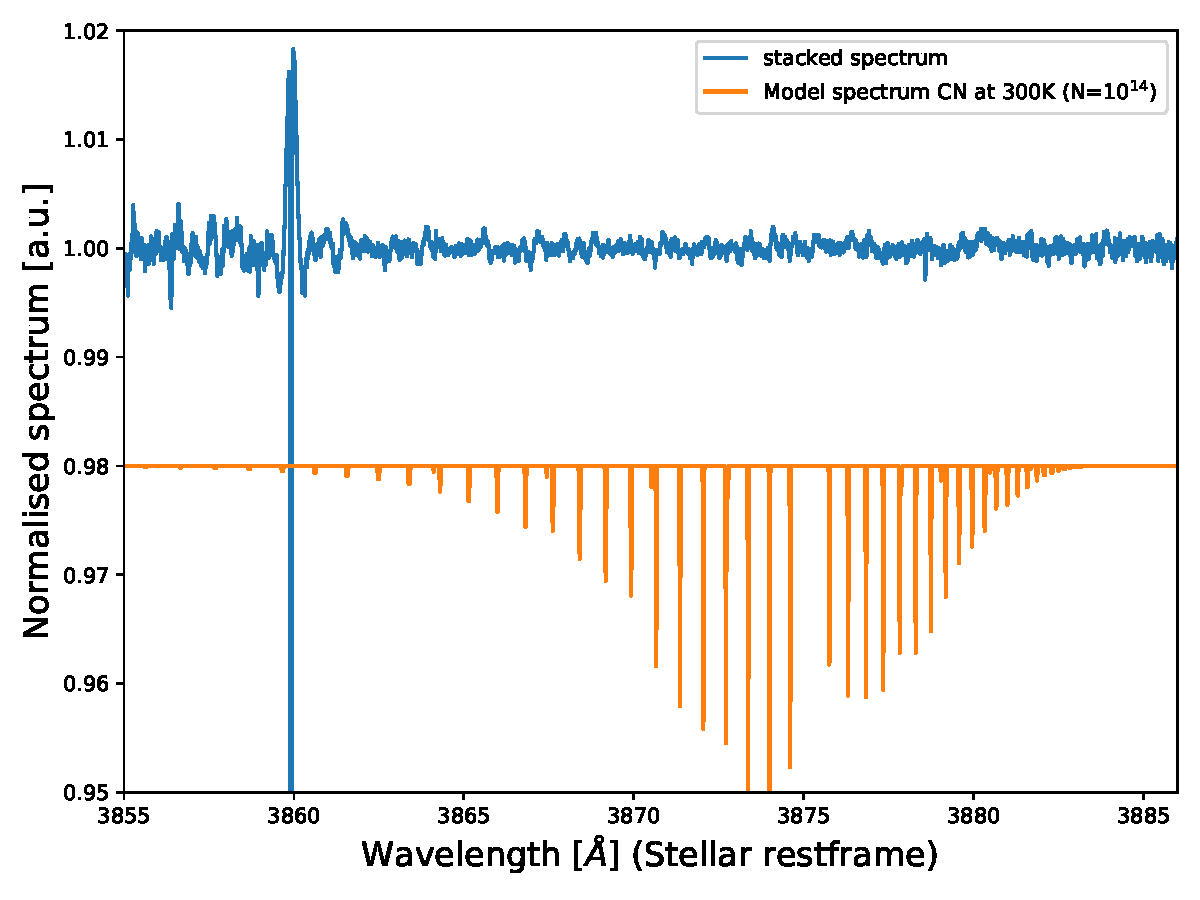
\includegraphics[width=\columnwidth]{figures/spec_stack_CN_stellar.pdf}
        \caption{Plot of the stacked spectrum in the stellar restframe (blue) with a CN model for $T=$300K and N=10$^{14}$\,cm$^{-2}$ overplotted in orange. The large signal around 3860\,\AA is due to the residual from a circumstellar \ion{Fe}{I} line.}
        \label{fig:spec_CN_stellar_frame}
        \script{plot_spec_mean.py}
    \end{centering}
\end{figure}


\begin{figure}
    \begin{centering}
        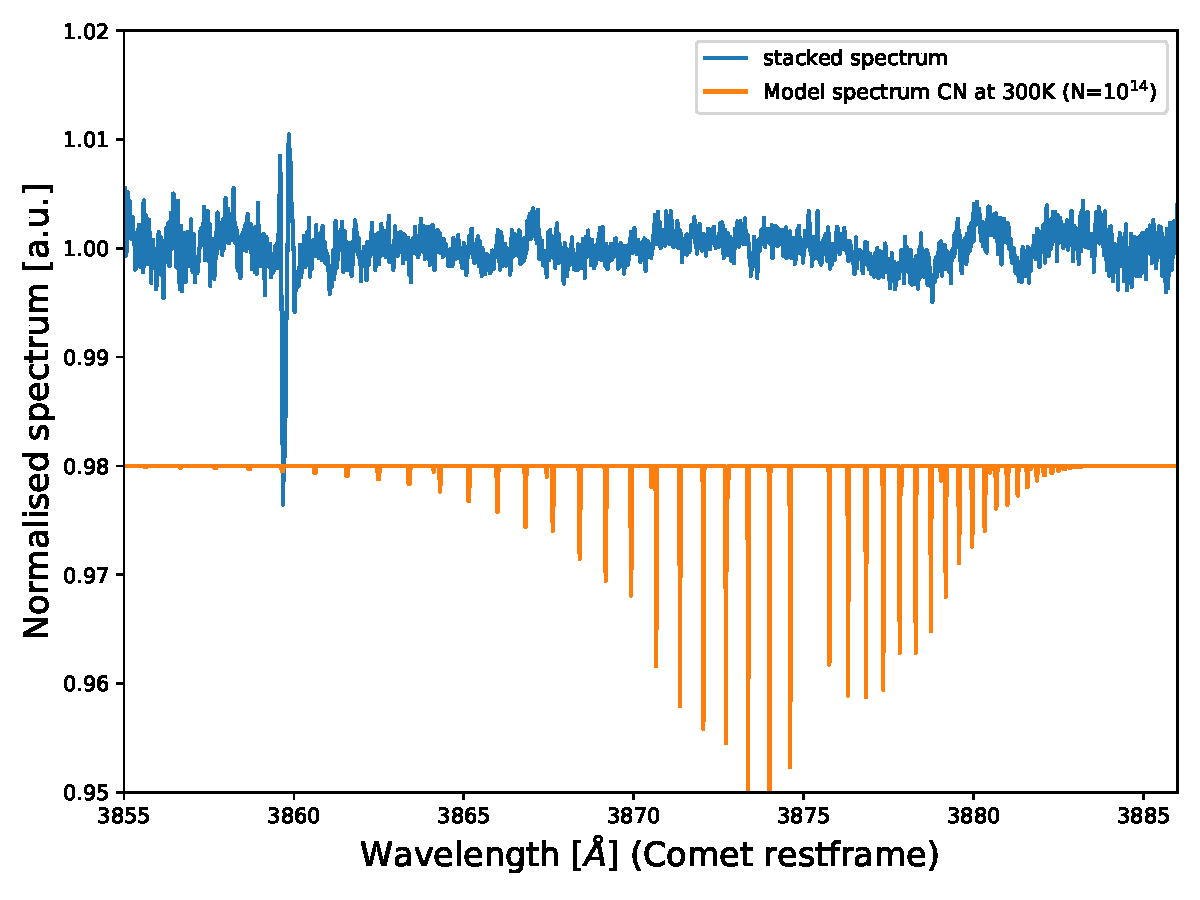
\includegraphics[width=\columnwidth]{figures/spec_stack_CN_comet.pdf}
        \caption{Plot of the stacked spectrum in the stellar rest frame (blue) with a CN model for $T=$300K and N=10$^{14}$\,cm$^{-2}$ overplotted in orange. The large signal around 3860\,\AA is due to the residual from a circumstellar \ion{Fe}{I} line.}
        \label{fig:spec_CN_comet_frame}
        \script{plot_spec_mean.py}
    \end{centering}
\end{figure}


\subsection{Cross-correlation with \ce{CN} models}\label{sect:CCF}


\begin{figure}
    \begin{centering}
        \includegraphics[width=\columnwidth]{figures/two_CN_temps.pdf}
        \caption{Model absorption spectrum for \ce{CN} at 30\,K (blue line) and 2000\,K (orange line). The  column densities are $N=10^{12}$\,cm$^{-2}$ and $N=10^{13}$\,cm$^{-2}$, respectively. }
        \label{fig:CN_theory}
        \script{plot_two_CN_temps.py}
    \end{centering}
\end{figure}

\begin{figure}
    \begin{centering}
        \includegraphics[width=\columnwidth]{figures/CN_ACF.pdf}
        \caption{\ce{CN} autocorrelation function for different temperatures. The aliasing at $\sim50$\,km\,s$^{-1}$ is clearly visible}
        \label{fig:CN_ACF}
        \script{plot_CN_ACF.py}
    \end{centering}
\end{figure}

To combine the signal from the many \ce{CN} lines, we cross-correlate the data for each night with a grid of model of \ce{CN}.
%
Cross-sections for \ce{CN} were obtained from ExoMol\footnote{\url{https://www.exomol.com}} \citep{Tennyson12,Tennyson16,Brooke14} with molecular energy levels assumed to be in thermal equilibrium, i.e.\ Boltzmann distributed.
%
We made models for a wide range of temperatures (T$=$\{10, 20, 30, 50, 100, 200, 300, 500, 1000, 2000, 3000\} K) and column densities\footnote{Note that technically, for optically thin lines, this assumes a filling factor $f=1$.
%
Since $f$ is unknown, we actually measure N$f$} (N=\{$10^{11} \ldots 10^{15}$\} cm$^{-2}$.
%
Each of the models was then convolved to include an effective velocity dispersion using a Gaussian for FWHM=\{2.9, 5, 10, 15, 20\} km\,s$^{-1}$.
%
A value of 2.9 km\,s$^{-1}$ corresponds approximately to the instrumental resolution of HARPS.
%
The theoretical spectra of \ce{CN} for several different temperatures are shown in Figure~\ref{fig:CN_theory}.

Even after cross-correlating, the stacked CCFs (see Fig.~\ref{fig:ccf_mean} do not show any clear signals, and we therefore proceed to estimate our detection limits.

\begin{figure}
    \begin{centering}
        \includegraphics[width=\columnwidth]{figures/FEB_velocity_depth.pdf}
        \caption{Peaks and radial velocities of exocomets identified in the stellar spectrum.
        %
        The peaks are normalised such that 1 represents total absorption in the spectrum.
        %
        Peaks closer than 10 km/s are masked out due to contamination from the circumstellar material.
        %
        Peak values above 0.6 are counted as exocomets and those below 0.15 as stellar only.}
        \label{fig:FEB_velocity}
        \script{plot_FEB_velocity_depth.py}
    \end{centering}
\end{figure}


\begin{figure}
    \begin{centering}
        \includegraphics[width=\columnwidth]{figures/ccf_mean.pdf}
        \caption{Cross correlation for different number densities of \ce{CN} averaged over many spectra.}
        \label{fig:ccf_mean}
        \script{plot_ccf_mean.py}
    \end{centering}
\end{figure}

\begin{figure}
    \begin{centering}
        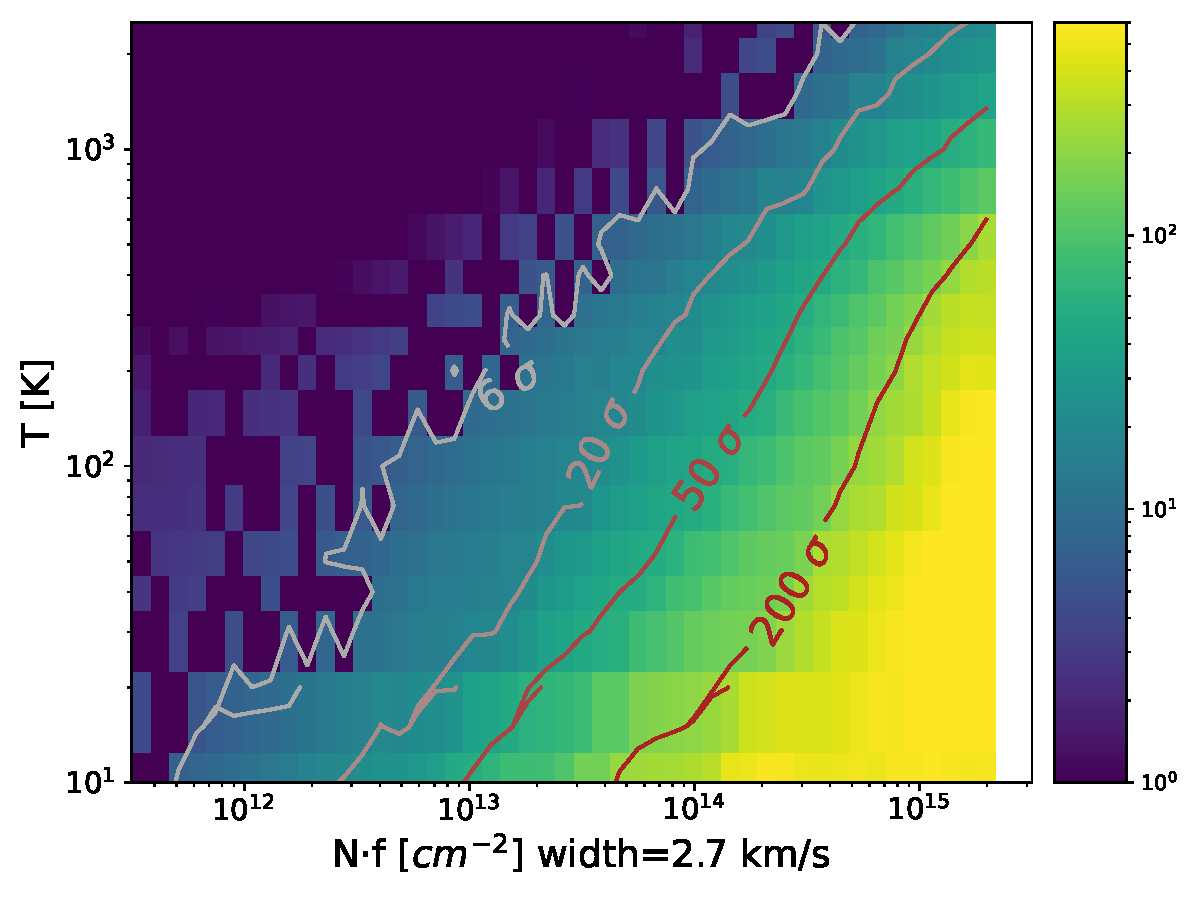
\includegraphics[width=\columnwidth]{figures/HARPS_CN_stellar_frame.pdf}
        \caption{\ce{CN} measurement limits in the stellar rest frame for a \ce{CN} line width of 2.7\kms{}. Contours show signal to noise upper limits.}
        \label{fig:CN_stellar_frame}
        \script{plot_HARPS_CN_stellar_frame.py}
    \end{centering}
\end{figure}



\begin{figure*}
    \begin{centering}
        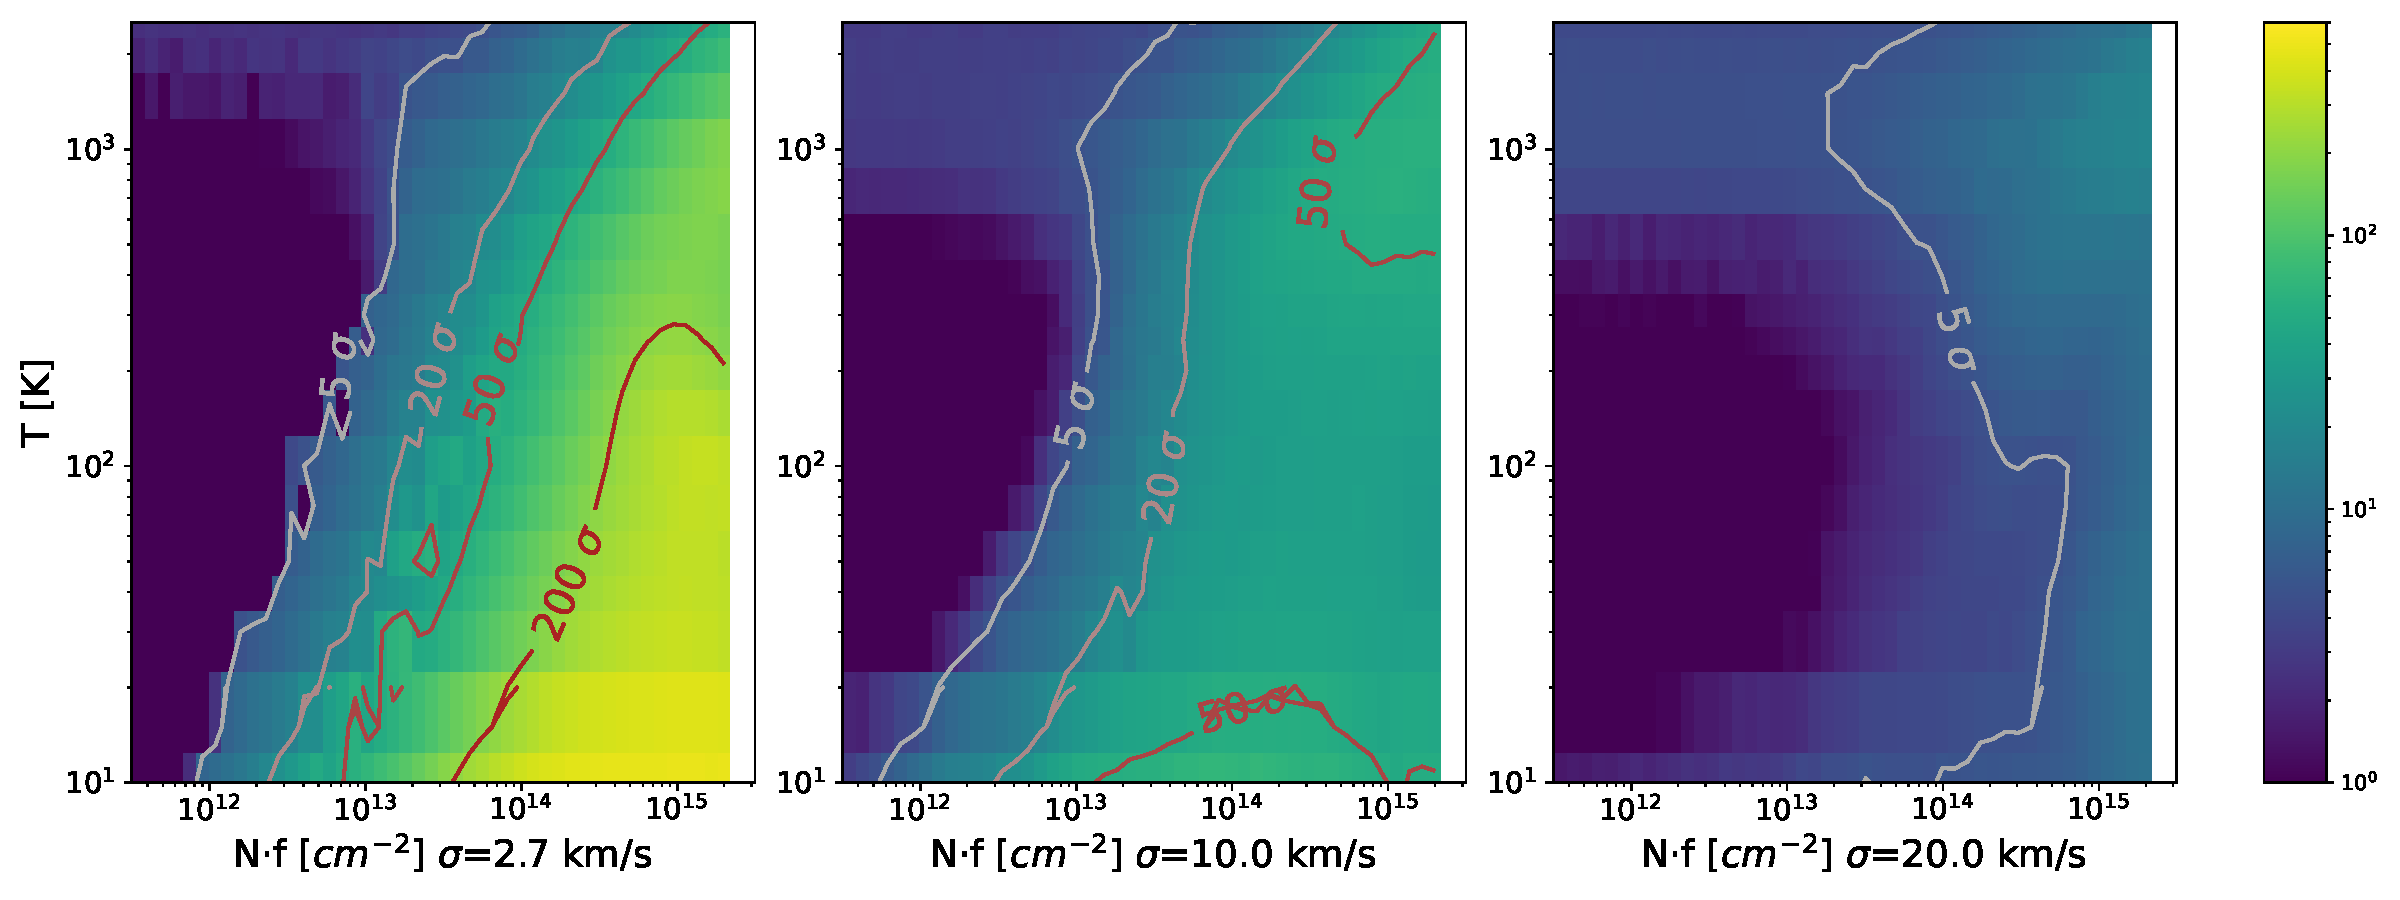
\includegraphics[width=\linewidth]{figures/HARPS_CN_exocomet_frame.pdf}
        \caption{\ce{CN} measurement limits in the exocomet frame for a \ce{CN} line width of 2.7, 10 and 20\kms{}. Contours show signal to noise upper limits.}
        \label{fig:CN_exocomet_frame}
        \script{plot_HARPS_CN_exocomet_frame.py}
    \end{centering}
\end{figure*}




% \begin{figure}
%     \begin{centering}
%         
\includegraphics[width=\columnwidth]{figures/asdf.png}
%         \caption{Test picture}
%         \label{fig:test}
%     \end{centering}
% \end{figure}


% \begin{figure}
%     \begin{centering}
%         \includegraphics[width=\columnwidth]{figures/HARPS_CN_grid.pdf}
%         \caption{Confidence intervals for the signal to noise of \ce{CN} spectra using \ac{harps} spectra of \bp{}.}
%         \label{fig:HARPS_CN_grid}
%         \script{plot_HARPS_CN_grid.py}
%     \end{centering}
% \end{figure}

%\subsection{Other Species? CO$^+$, C$_2$?}

\subsection{Estimating the \ce{CN} column density limits}\label{sect:CNlim}

To estimate the limits on the \ce{CN} detection, we perform injection and recovery tests.
%
We injected models for different temperatures, column densities and velocity broadening into the nightly stacked spectra (Sect.~\ref{sect:comb}), and then processed them in the same way as the original data (i.e., correct for residual blaze variations, removal of the stellar envelope and cross-correlation).
%
This was done for all spectra with the injected signal in the stellar rest frame as well as for the sample of spectra with strong cometary activity in the rest frame of the strongest exocometary feature per night.

The individual CCFs show some overall slopes and offsets, and we fit each individual CCF with a combination of a second-order polynomial baseline and a Gaussian with the position fixed to 0 \kms{} in its rest frame.
%
The fit has five free parameters: the amplitude of the peak, the width of the peak, and the offset, slope, and intercept of the baseline.
%
To avoid the aliasing peaks of the \ce{CN} band (see Figure~\ref{fig:CN_ACF}), we only fit the central $\pm$35 \kms{} of the CCF.
%
Fitting is done using the curve\_fit function from SciPy \citep{2020SciPy-NMeth}.
%
We correct each of the individual CCFs for the baseline and then stack the corrected CCFs to obtain our master CCF that we use for determining the upper limit.
%
The noise on each point in the master CCF is determined by taking the standard deviation in time for each pixel and dividing that by the square root of the number of points.

This master CCF is then fitted in the same way as the nightly CCFs, and the uncertainties on the parameters is taken directly from {\tt curve\_fit} assuming no covariance between the parameters.
%
The final detection significance for the injected models is determined by the amplitude divided by its uncertainty, and shown in Figure~\ref{fig:CN_stellar_frame} for the circumstellar gas and in Figure~\ref{fig:CN_exocomet_frame} for the strongest exocomet features.

\section{Discussion}\label{sec:discuss}

%\subsection{Summary of \ce{CN} in comets}
%\ce{CN} is one of the brightest optically active species in cometary comae.
%
%It is a minor component of the gas coma, with a production rate by number $\sim 1/500$th that of water. 
As discussed above in the introduction, most studies of Solar system comets observe the \ce{CN} molecules via optical fluorescence. From measurements and simple physical arguments the \ce{CN} absorption/emission is optically thin everywhere.
This means a flux from part of the coma can immediately be converted to a column density using a photon scattering efficiency for the molecular band.

\ce{CN} in solar system comets comes from two sources.
Sublimation of nucleus near-surface ices releases \ce{HCN}, which then photo-dissociates into \ce{CN}.
This in turn eventually photo-dissociates into the component atoms.

$$\ce{HCN} +\gamma \rightarrow \ce{H}+\ce{CN}$$
$$\ce{CN} + \gamma \rightarrow \ce{C}+\ce{N}$$

Since observations of Comet Halley \citep{AHearn1986}, it has also been known that dust grains ejected from the nucleus also directly release \ce{CN} into the coma.
However, \ce{CN} production in comets is usually dominated by nuclear ice sublimation \citep{Fray2005}. The resulting \ce{CN} coma will have a true space density and apparent column density distribution centrally peaked at the comet nucleus in this case.

For Solar system comets, measured \ce{CN} column densities are often converted to an overall production rate by the comet of $Q_{\ce{CN}}$ molecules/sec via an analytical model known as the ``Haser'' model \citep{Haser2020}
This model gives the on-sky column density as a function of projected radial distance form the nucleus using only 3 parameters; the effective destruction scale length $l_p$ of the parents of \ce{CN} (\ce{HCN}+dust), the photodissociation scale length $l_{\ce{CN}}$ of \ce{CN}, and the gas outflow velocity $v$. The Haser model is somewhat simplistic but it represents the data well for solar system comets observed at typical distances from the Sun (1--3 au).

\subsection{Example comet - 1P/Halley}

We take the observed activity of 1P / Halley in 1985 / 1986 as a reference point for our estimates.
%
Although most Solar system comets are observed to be are far less active than Halley, some Long-Period comets show activity in excess of Halley.
Given that we will be dominated by the most active comets at \bp{}, this seems reasonable as something that can be later scaled to the most active comets such as Hale-Bopp \citep{Schleicher2024}.
%
When Halley was at $\sim 1$ au from the Sun, it was measured to have $Q_{\ce{CN}}\simeq 10^{27}$ molecules/sec using Haser models \citep{AHearn1995}.
%
The assumed outflow velocity in the models was generally  $0.85 - 1$ \kms{} at this distance.

For solar system comets, the normal Haser scale lengths used are \citep{Cochran86,AHearn1995} :

$$lp=1.7\times10^4r_h^2\:{\rm km}$$
$$l_{\ce{CN}}=2-3\times10^5r_h^2\:{\rm km}$$

Both are assumed to scale with heliocentric distance $r_h^2$ as photodissociation or thermal desorption is assumed the main physical pathway for both the parent and \ce{CN}.

The lifetime of \ce{HCN} for photodissociation into \ce{H}+\ce{CN} at 1~au has been calculated to be $(3.2-7.7)\times10^4$ sec, with lifetime of \ce{CN} dissociating into \ce{C}+\ce{N} being $(1.3-3.1)\times10^5$ sec \citep{Huebner92}, depending on solar activity levels.
%
These are consistent with the measured scale lengths above if the parents of \ce{CN} are ejected at $\sim 0.5$ km/sec, and we take into account the excess photodissociation energy giving \ce{CN} an extra kick of $\simeq1$ \kms{} \citep{Combi1980}. 

\subsection{1P/Halley at \bp{}}

%\subsubsection{Total \ce{CN} Abundance}

Photodissociation is  driven by the UV photon flux at the comet, which in turn is dominated by Ly-$\alpha$ line flux. From Ly-$\alpha$ measurements in \citet{Landsman93} the intrinsic Ly-$\alpha$ luminosity of A6V/A7V stars is a factor of $\sim10$ higher than for G2V stars.
%
Hence the photodissociation lifetime of \ce{CN}  at 1 au from \bp{} of an `exoHalley' will be approximately 10 times smaller i.e. $\sim 2\times10^4$ sec at 1 au.

In steady-state sublimation, the sublimation rate is proportional to the photon flux at the comet. For \bp{} $L=8.7L_\odot$, so assuming 
all \ce{CN} production scales with stellar luminosity, exoHalley would have a larger \ce{CN} production rate of $Q_{\ce{CN}}\sim 9\times10^{27}$ molecules/sec.
%
The total number of \ce{CN} molecules in the coma at 1~au at any given time would therefore be

$$N_{\ce{CN}}=Q_{\ce{CN}} \tau_{\ce{CN}}$$
$$N_{\ce{CN}}\sim 9\times10^{27} \cdot  2\times10^4 \sim 2\times10^{32}\:{\rm molecules}$$

%\subsubsection{\ce{CN} Cross-section}
The effective cross section of the coma will depend on how much is projected against the disk of \bp{}. The radius of the \ce{CN} coma will be given by
$$r\sim v_{\ce{CN}} \tau_{\ce{CN}}$$.
The outflow velocity of the parent \ce{HCN} will depend on the nuclear surface temperature, which will increase as a comet moves towards its parent star.
\citet{Biver2002} found a nuclear gas outflow velocity $v\simeq1.0  r_h^{-0.4}$ \kms{} from sub-mm measurements of Comet Hale-Bopp, close to the canonical relationship of $r_h^{-0.5}$.
\citet{Harris2002} notes lower activity similar to Halley results in smaller outflow velocities.
%Dust grains will also be travelling faster due to the larger gas pressure accelerating them.
The excess photodissociation velocity of \ce{CN} will not change.
Therefore gas outflow speeds are expected to be $\sim 1-2$ \kms{} at 1 AU, and the \ce{CN} coma radius will be
%
$$r\sim (1-2) \times 2\times 10^{4} \leq 4\times 10^{4}\:{\rm km}$$
This is much smaller than a stellar radius, so we can assume for an exoHalley that all of the coma is projected into the stellar disk as seen from Earth.

\bp{} has $R=1.8R_\odot\equiv 1.3\times 10^{11}$ cm.
%
Given that the coma is optically thin, and we do not resolve the star, the effective average column density towards \bp{} is 

$$n\sim\frac{N_{\ce{CN}}}{\pi R_*^2}$$

$$n\sim\frac{2\times10^{32}}{\pi\cdot 1.7\times10^{22}}\sim 3\times10^{9}\:{\rm cm^{-2}}$$
Therefore an exoHalley at 1~au from \bp{} would result in a \ce{CN} column density of $10^{9}-10^{10}$ cm$^{-2}$.
%
This is about a factor of 100 smaller than our measured upper limits above.

\subsection{Raising the \ce{CN} production rates}

%\subsubsection{We need a bigger comet}
There are several ways exocomets at \bp{} may exhibit larger \ce{CN} production rates.
%
A larger comet gives more surface area for sublimation.
%
 Comet Halley's nucleus has an effective radius of $5.5$ km \citep{Keller1987}, whereas 
Comet Hale-Bopp was one of the most intrinsically active comets on record with an extremely large nucleus of radius $\sim 14-21$ km \citep{Weaver1997}.
%
However most of the apparent brightness was due to dust emission, and its only had $Q_{\ce{CN}}\simeq 3\times10^{27}$ molecules/sec \citep{Schleicher2024}.
%
In this case, we might anticipate the most active comets in the Solar system to have $Q_{\ce{CN}}\sim 10^{28}$ molecules/sec, implying a commensurate increase of a factor 10 in column density $n$ over an exoHalley at \bp{}.

%\subsubsection{Turn on the taps}

Most comets only have a fraction of their surface area undergoing mass-loss, due to the effect of a thermally insulating dust crust.
%
Halley itself only has $\sim20$\% of the sunlit surface active \citep{Keller1987}.
%
Yet some comets are known as hyperactive, as the measured gas productions rates would require $\geq 100$\% of the nucleus surface to be active \citep{Sunshine2021}. This is believed to be due to the release of ice-rich dust grains from the nucleus, which sublimate and act as a secondary source of gas.
Assuming this is possible for exocomets at \bp{} would increase $N_{\ce{CN}}$ and $n$ by a factor $\sim 5$.

%\subsubsection{Move it closer to \bp{}}

The closer a comet to its parent star, the greater the heating and corresponding production rate. When insolation completely controls the nuclear surface energy balance we expect
$Q_{\ce{CN}}\propto r_h^{-2}$.
%
Studies of Halley and Hale-Bopp showed power laws close to this {\it i.e.} \cite{Biver2002}. But the photodissociation lifetime $\tau_{\ce{CN}}\propto r_h^{2}$, so theoretically
$$N_{\ce{CN}}=\frac{Q_{\ce{CN}}(1~\rm{au})}{r_h^2}\cdot  \tau_{\ce{CN}} (1~\rm{au}) r_h^2 =\:{\rm constant} $$
Hence the total amount of \ce{CN} in the coma should be approximately independent of stellar distance, and the total cross-section would not change.

%\subsubsection{Stay up all night to get lucky}
Finally, comets have impulsive outbursts, where the amount of material ejected into the coma increases significantly over a few hours or less.
%
%This varies from comet to comet; many do not appear to outburst, some have 1 or a few outbursts per orbit.
%
The general causes are unclear, but there is evidence for several physical mechanisms that cause them 
\citep{Kelley2021,Muller2024}.
``Normal'' outbursts generally result in a brightness increases of 1--5 magnitudes, with smaller outbursts being more common.
%
As the apparent brightness is directly proportional to the amount of material (gas+dust) in the coma, this implies short term increases in $N_{\ce{CN}}$ and $n$ of factors $\sim 2-100$.

Large outbursts are often due to partial or total disruption of a comet and can occur when a comet is closer to the Sun.
Hence there could be a correlation with faster moving \bp{} exocomets nearer their periastra producing greater measurable column densities of \ce{CN}.

In summary, mechanisms exist by which the \ce{CN} column density of an exocomet at \bp{} could exceed $n\sim10^9-10^{10}$ cm$^{-2}$. 
A larger and/or hyperactive nucleus could increase $n$ by a factor 10. Even larger increases are possible with an outburst or comet disruption, but the upper boundary is likely to be near $n\sim10^{12}$ cm$^{-2}$. 

\section{Conclusions}\label{sec:conclusion}

We have combined over 1000 spectra of \bp{} over a 20 year period, identified two groups, one with deep exocomet signals, and another to act as a stellar reference.
%
We produce a normalised spectrum towards \bp{} with the stellar spectral features removed, and then aligned the spectra to the exocomet rest frames and perform a search for \ce{CN} using cross correlation.

We do not detect \ce{CN} both in the stellar rest frame and in the exocomet rest frame.
%
Injection and recovery tests show that for the circumstellar \ce{CN} we are sensitive to $10^{12.5}$ cm$^{-2}$ below 80~K and below $10^{14}$cm$^{-2}$ up to 1800~K.
%
In the exocomet rest frames, sensitivity is somewhat similar.
%
Below 100K the sensitivity is $10^{12}$cm$^{-2}$ and above from 100 - 1800~K, is $10^{13}$cm$^{-2}$.
%
This is a factor of 10 to 100 too high to detect a single Hale-Bopp equivalent comet with a \ce{CN} coma.
%
%We detect no \ce{CN} absorption, but can place five sigma upper limits of 10e12 to 10e13 from 10 to 1800 K.
%
%Hale-Bopp in transit will be around $10^{10}$, so we are two orders of magnitude above this in our detection.
%
The assumptions are for steady state comets, so individual outbursts could build this number up, and multiple transiting exocomets can increase the absorption cross section.

\bp{} is the brightest star with known exocomets seen both in transit and spectroscopy, and represents the best candidate for exocomet characterisation.
%
A more dedicated observing campaign over several years using dedicated spectrographs can reach the equivalent Solar system limits for \ce{CN}.
%
PLATO will carry out a dedicated long stare campaign that will observe the star with sub-millimagnitude photometry over 2 to 3 years.
%
This presents an excellent opportunity for coordinated spectroscopic campaigns where the exocomet population of \bp{} can be characterised, with \ce{CN} and ideally other molecules known from Solar system comets to be identified in another stellar system.

\begin{acknowledgements}

The authors thank the Lorentz Centre at Leiden University for organising the workshop ``Exocomets: Understanding the Composition of Planetary Building Blocks'' which led to the study in this paper. 
%
Part of this work was supported by the German \emph{Deut\-sche For\-schungs\-ge\-mein\-schaft, DFG\/} project number Ts~17/2--1.

AF acknowledges support from STFC award ST/T00021X/1. EdM acknowledges support from STFC award ST/X00094X/1.
%
We made use of the {\tt Python} programming language \citep{rossum1995} and the open-source {\tt Python} packages {\tt numpy} \citep{walt2011}, {\tt matplotlib} \citep{hunter2007}, {\tt astropy} \citep{astropy2013}.
%      
An online repository with materials used in this work is available at \url{https://github.com/mkenworthy/BetaPicCN}

\end{acknowledgements}

\bibliographystyle{aa}
\bibliography{bib.bib}

\end{document}
